\chapter{Advanced Techniques}

\section{Copy and Paste} \label{copy-paste}

Little Sound Dj has a clipboard for temporary data storage. Pressing \textsc{b+a} will cut the value
under the cursor and store it on the clipboard. The value can then be pasted by pressing
\textsc{select+a}.

In most screens, it is possible to mark up blocks by pressing \textsc{select+b} and moving around
the cursor. When having marked up a block, it can be copied to the clipboard by pressing \textsc{b},
or cut to the clipboard by pressing \textsc{select+a}. The clipboard contents can then be pasted by
pressing \textsc{select+a}.

Some quick-mark button presses are implemented:
\begin{itemize}
\item \textsc{select+(b, b)} = quick-mark a column or row.
\item \textsc{select+(b, b, b)} = quick-mark an entire screen.
\end{itemize}

When having marked a block, you can change all data inside that block by pressing \textsc{a+cursor}. This can be used, for example, to transpose several notes quickly.

\section{Cloning} \label{cloning}

Cloning is a shortcut that can save you much unnecessary copy and paste work.
It allows you to create copies of chains, phrases, instruments and tables directly from the song, chain, phrase and instrument screens.

Let's imagine you want to make a slightly altered version of the melody in chain 0. Go to the song screen, tap \textsc{a} on 00 to pick the number, then tap \textsc{a} again on a down-below empty step so that you get:

\begin{verbatim}
 00
 00
\end{verbatim}

Now, move the cursor to the second 00 and press \textsc{select+(b, a)} to make a copy of chain 0.

\subsection{Deep vs. Slim-Cloning}

There are two different cloning modes: deep and slim cloning, selectable from the project screen.

When slim-cloning a chain, a new chain appears that contains the same phrases as the original.

When deep-cloning a chain, a new chain appears with copies of the original phrases.

The advantage of deep-cloning is that you lessen the risk of modifying old phrases by accident.
The drawback is that will run out of phrases faster.
Also, your songs might take up more space when saved in the file screen.

If you run out of phrases, use \textsc{clean song data} in project screen. (Section \ref{clean-song-data}.)

\section{The Importance of Backups}

Some words of caution from many peoples hard-earned experience: When using a Game Boy cartridge, backup your songs! Most Game Boy cartridges depend on an internal battery that will run out, losing your songs in the process. If you care about your music, do regular backups, or at least record your songs to prevent them from being lost forever.

\section{Muting, Soloing and Panning}

\begin{itemize}
\item Press \textsc{b+select} in any screen to mute the channel. If the \textsc{b} button is released before \textsc{select}, the channel stays muted until \textsc{b} is pressed again.
\item Press \textsc{b+start} in any screen to solo the channel. If the \textsc{b} button is released before \textsc{start}, the other channels stay muted. If the \textsc{start} button is released first, all channels will be turned on again.
\item Press \textsc{b+left/right} in the song screen to pan a channel left or right.
\end{itemize}

\section{Live Mode}

Live mode is ideal to freely mix and match chains during a live performance.

Song screen controls:

\begin{description}
	\item[\textsc{Select+Left}] Switch between song and live mode
	\item[\textsc{Start}] Start selected chain(s)
	\item[\textsc{Select+Start}] Stop selected chain(s)
	\item[\textsc{Left+Start}] Start all chains in the row
\end{description}

If a chain is already playing, starts and stops are queued until the chain played through.
Pressing \textsc{Start} twice speeds up the change so that it happens already when the active phrase played through.

\section{Synthetic Drum Instruments}

Creating drum instruments without using the sampled drum kits can be very useful, as it gives greater flexibility in how to make use of the channels. Here are some starting-out ideas.

\begin{figure}[hbtp]
	\centering
	\subfloat[Bass Drum]{
		\fbox{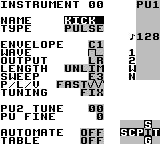
\includegraphics{instr-kick}}
	}
	\qquad
	\subfloat[Snare Drum]{
	\fbox{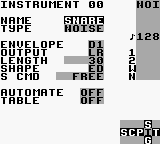
\includegraphics{instr-snare}}
	}

	\subfloat[Closed Hi-Hat]{
		\fbox{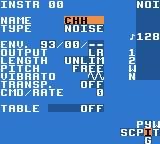
\includegraphics{instr-chh}}
	}
	\qquad
	\subfloat[Open Hi-Hat]{
	\fbox{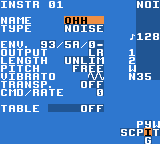
\includegraphics{instr-ohh}}
	}

	\subfloat[Cymbal]{
		\fbox{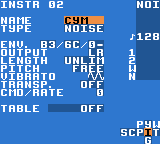
\includegraphics{instr-cym}}
	}

	\caption{Synthetic Drum Instruments}
	\label{fig:instr-examples}
\end{figure}

\subsection{Pulse Bass Drum}

The easiest way to create a bass drum is by using pulse channel 1. \textsc{Env.} should have a strong attack and fast decay -- try setting it to C3/0/0. \textsc{Wave} is typically 50-50 high/low, even though other waves can be used for a more distorted sound. \textsc{Sweep} should have high initial frequency and fast decay; try setting it to 63, and play the instrument at note C-6. For a snappier kick, experiment with \textsc{env.} and \textsc{length} parameters. Set \textsc{transpose} to \textsc{off} to prevent chain transposes from changing the pitch.

\subsection{Snare Drum}

Use the noise channel for snare drum sounds. The \textsc{env.} setting should have a strong attack and fast decay -- try setting it to F1/D3/0.
Adjust the timbre by changing note value in phrase screen. Note values around 30 should be useful for snares.
\textsc{P} and \textsc{v} commands can help making the sound more lively.

\subsection{Hi-Hats and Cymbals}

Use the noise channel for hi-hats and cymbals. Use a phrase note value around 38 for a timbre with high frequency content. Change instrument \textsc{env.} to get the desired amplitude envelope. For cymbals, lower the notes a bit for a rougher timbre.

\begin{figure}[hbtp]
	\centering
	\subfloat[Bass Drum Instrument]{
		\fbox{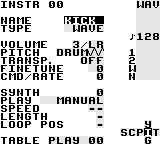
\includegraphics{instr-wavekick}}
	}
	\qquad
	\subfloat[Bass Drum Synth]{
	\fbox{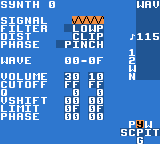
\includegraphics{synth-wavekick}}
	}

	\subfloat[Bass Drum Wave]{
		\fbox{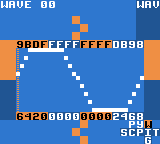
\includegraphics{wave-wavekick}}
	}
	\qquad
	\subfloat[Bass Drum Table]{
	\fbox{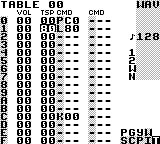
\includegraphics{table-wavekick}}
	}

	\caption{Wave Channel Bass Drum}
	\label{fig:wavekick}
\end{figure}

\subsection{Wave Bass Drum}

For the best sounding bass drum, use the synthesizer in the wave channel. Set the \textsc{pitch} to \textsc{drum} by pressing \textsc{a+up}, and set \textsc{transp.} to \textsc{off}. On the synth screen, choose the triangle signal, and set \textsc{volume} to 30. Set a table for the instrument. On step 0 of the table, use a fast P command such as C0. On line 1, put 80 in the \textsc{tsp} column and use an L command with a value such as 30. This will transpose the bass drum to the lowest possible note without wrapping to a higher pitch.  Feel free to experiment with different synth parameters or different values for the P and L commands to shape the sound of the kick, as well as playing the instrument at note C-5, C-6, or above. (See figure~\ref{fig:wavekick}.)
